\documentclass[12pt]{article}

\usepackage{math}

\begin{document}
\begin{flushleft}

\setlength{\parindent}{30pt}


\intro{2-Polytopes}{Feb. 19, 2023}{}


\section{Introduction} 

Let $M$ be a two-dimensional convex and compact polytope in $\R^2$.
We will also assume that $M$ is \textit{non-degenerate}, in the sense that the internal angle at each vertex is less than $\pi$.

In this problem, the polytope $M$ is unknown.
We are given an \textit{oracle} that returns the signed (minimum) distance from a point $x\in\R^2$ to the boundary of $M$.
That is, our oracle is the function
\begin{align*}
	\F: \R^2 &\to \R\\
	x &\mapsto d(x,\partial M)
\end{align*}
where $d:\R^2\to \R$ is the signed Euclidean distance function, where distance is positive for points outside $M$ and negative for points inside $M$.
Our goal is to use the oracle to identify the unknown polytope $M$.

The overall strategy will be to pick sample points in $\R^2$ and evaluate their distance from the polytope using the oracle.
Given a point $x_i\in\R^2$, we will write $R_i=\F(x_i)$ as its distance from $M$.
We then have a circle $S_i$ centered at $x_i$ with radius $R_i$ that contains exactly one point of $M$.

\begin{figure}[H]
	\centering
	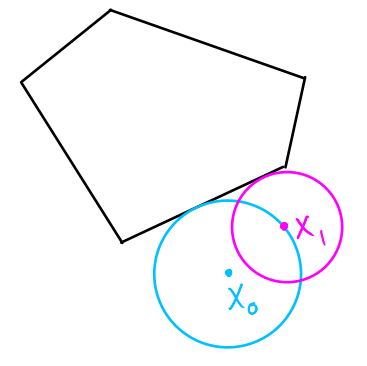
\includegraphics[width=0.4\textwidth]{1.png}
\end{figure}

\begin{prop}{1}
	For any $x_i\in\R^2$, the circle $S_i$ centered at $x_i$ with radius $R_i$ intersects $M$ in exactly one point.
\end{prop}
\begin{proof}
	Recall that the radius $R_i$ of $S_i$ is constructed to be the minimum distance from $x_i$ to the polytope $M$.
	Suppose $S_i$ contains two points $p$ and $q$ of $M$.
	Since $M$ is convex, $M$ contains the straight line segment $\ell$ containing $p$ and $q$.
	But $\ell$ is a chord in $S_i$ and so contains points of $M$ closer to $x_i$ than $p$ and $q$, which is a contradiction.
\end{proof}


\section{Identifying Points and Edges}

\begin{defn}
	Let $e$ be an edge of the polytope $M$.
	The \textbf{domain} $\dom(e)$ of $e$ is the set of points in $\R^2$ whose minimum distance to $M$ is positive and is equal to the distance to $e$.
	That is,
	\[\dom(e) = \set{x\in\R^2 \st \F(x) = d(x,e) \andt \F(x)>0}.\]
	The \textbf{domain} $\dom(p)$ of a point $p$ is defined similarly.
\end{defn}

\begin{figure}[H]
	\centering
	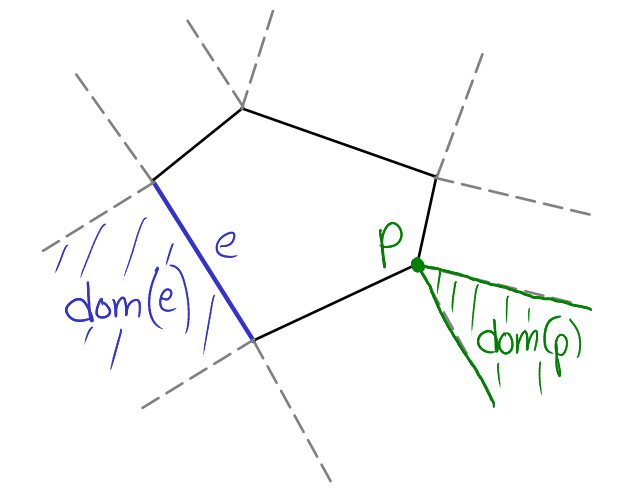
\includegraphics[width=0.4\textwidth]{2.png}
\end{figure}

We will view each edge $e$ of $M$ as an open line segment.
The domain of $e$ is then an open subset of $\R^2$ bounded by $e$ and the two lines normal to $e$ starting at the endpoints of $e$.
The domain of a point $p$ is the closed cone bounded between the lines normal to the two edges containing $p$.

In what follows, we will adopt the following strategy for selecting sample points in $\R^2$.
First we will select an arbitrary point $x_0$ that lies outside $M$, so $R_0>0$.
Using the oracle, we consider the circle $S_0$ that touches the unknown polytope $M$ at exactly one point.
We will randomly choose a point $x_1$ that lies on $S_0$.

The geometry of the two circles $S_0$ and $S_1$ will give us clues as to which domains the points are in.
Note that since $x_1\in S_0$, the circles $S_0$ and $S_1$ will always intersect in at least one point.

\begin{prop}{2}
	Let $x_0,x_1\in \R^2$ with $x_1\in S_0$.
	Suppose that $S_0\cap S_1 = \set{p,q}$ where $p\neq q$.
	If $\F(p)=0$ then $p$ must be a vertex of $M$.
\end{prop}

\begin{figure}[H]
	\centering
	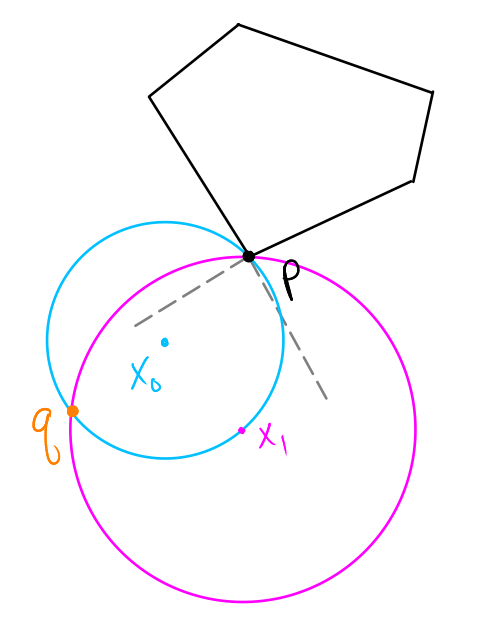
\includegraphics[width=0.4\textwidth]{3.png}
\end{figure}

\begin{proof}
	Suppose that $\F(p)=0$ but $p$ is not a vertex of $M$, and so lies on an edge $e$.
	By \textit{Proposition 1} $p$ is the only point of $M$ that lies on both $S_0$ and $S_1$.
	The edge $e$ is then tangent to both $S_0$ and $S_1$ at $p$.
	But two intersecting circles that share a tangent line at a point must either be equal or share one intersection point.
	In either case we have a contradiction.
\end{proof}

\begin{prop}{3}
	Let $x_0,x_1\in \R^2$ with $x_1\in S_0$ and suppose $S_0\cap S_1=\set{p,q}$ where $p\neq q$ and $\F(p)<\F(q)$.
	Let $\ell$ be the common tangent line to both $S_0$ and $S_1$ closest to $p$.
	Then there exists at least one sub-segment of an edge of $M$ contained within the region $R$ bounded by $\ell, S_0$, and $S_1$ (including possibly the boundary of this region).
\end{prop}

\begin{figure}[H]
	\centering
	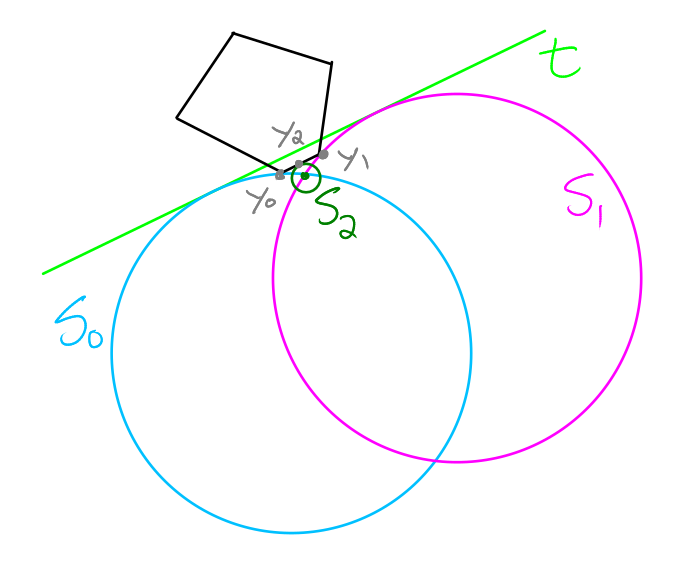
\includegraphics[width=0.4\textwidth]{4.png}
\end{figure}

\begin{proof}
	By \textit{Proposition 1}, $M$ intersects each of $S_0, S_1,$ and $S_2$ in exactly one point. 	
	Say that $S_i$ intersects $M$ at $y_i$ and suppose that $y_2$ lies outside the region $R$. 
	Since $M$ is a convex polygon, there is a sequence of edges from $y_0$ to $y_2$ and from $y_2$ to $y_1$.
	But if $y_2$ lies outside of $R$, this sequence of edges must cross $\ell$ more than twice.
	Since any line that crosses through the interior of a convex polygon intersects the edges of the polygon exactly twice, this is a contradiction.
\end{proof}


Let $\epsilon>0$ be a ``small'' user-defined parameter that will represent the accuracy of the accuracy tolerance of the algorithm.
We will utilize $\epsilon$ in such a way that edges of $M$ that have length smaller than $\epsilon$ will not be found.

Our first step in identifying portions of the boundary of $M$ is to first find any single point on the boundary. 
This initial stage of the algorithm reduces to one of several cases.

\textbf{Case 1.} 
Suppose that $S_0\cap S_1=\set{p}$.
Then if $p$ is interior to an edge $e$, that edge is determined by the line $t$ containing $p$ that is orthogonal to the line containing $x_0$ and $x_1$.
If $p$ is instead a vertex, we may still use the line $t$ to determine the adjacent edges.

We may take the line $t$ as an axis of a coordinate system with $p$ at the origin and pick two points $p+\epsilon$ and $p-\epsilon$ that are a distance of $\epsilon$ from $p$ along $t$.
If $\F(p\pm\epsilon)=0$, then that point lies exactly on an edge determined by the line containing $p$ and $p\pm\epsilon$.
Otherwise, under the assumption that no edges of $M$ have length smaller than $\epsilon$, the points $p\pm\epsilon$ are in the domains of edges containing $p$.
Therefore we may find an edge to be the line containing $p$ that is tangent to $S_{p\pm\epsilon}$.

\begin{figure}[H]
	\centering
	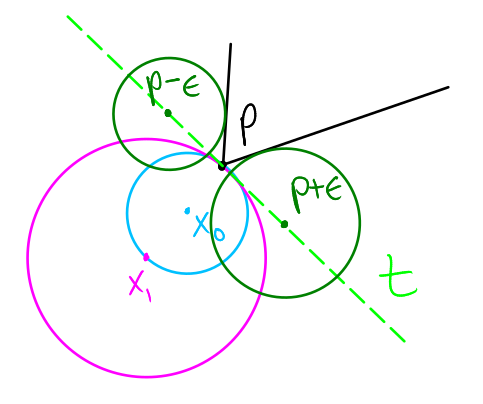
\includegraphics[width=0.4\textwidth]{5.png}
\end{figure}
\begin{figure}[H]
	\centering
	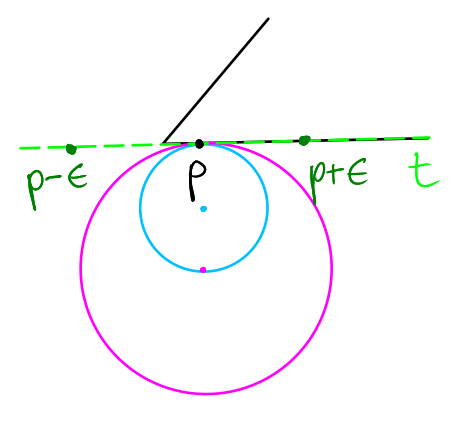
\includegraphics[width=0.4\textwidth]{6.png}
\end{figure}

\textbf{Case 2.}
Suppose now that $S_0\cap S_1=\set{p,q}$ where $p\neq q$, and say that $\F(p)=0$.
Then we know that $p$ is a vertex of $M$ by \textit{Proposition 2}, and we seek to find the edges containing $p$.
Let $\ell_0$ be the line tangent to $S_0$ containing $p$ and choose a point $p+\epsilon_0$ on $\ell_0$ a distance $\epsilon$ away from $p$ in the direction away from $S_1$.
Then we may find an edge to be the line containing $p$ that is tangent to $S_{p+\epsilon_0}$.
Similarly, we may find the other edge containing $p$.

\begin{figure}[H]
	\centering
	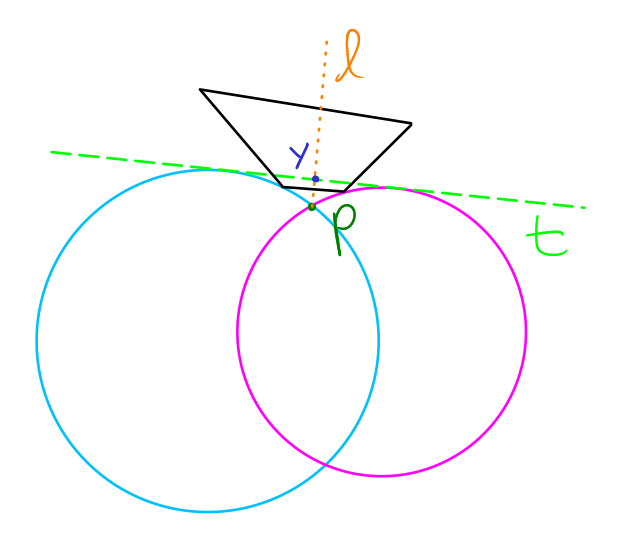
\includegraphics[width=0.4\textwidth]{7.png}
\end{figure}

\textbf{Case 3.}
Assume that $S_0\cap S_1=\set{p,q}$ where $p\neq q$ and $\F(p)<\F(q)$.
By \textit{Proposition 3} there exists a sub-segment of an edge of $M$ contained within the region $R$ bounded by $S_0$, $S_1$, and the common tangent line $t$ to both $S_0$ and $S_1$.
Consider the line $\ell$ through $p$ that is orthogonal to $t$ and let $y$ be the intersection of $t$ and $\ell$.
Note that by convexity of $M$, $\ell$ intersects $M$ in either one or two points.
We aim to find the closest intersection point to $p$.
This can be done by a linear or binary search using the oracle along the line $\ell$, starting at $y$.
Note that $\F(y)=0$ when the tangent line $t$ contains an edge of $M$.
Once the closest intersection point $z$ is found, we choose the axis to be aligned with a line $t'$ parallel to $t$ that passes through $z$.
We may then find the edges containing/adjacent to $z$ by stepping along the axis by a distance of $\pm\epsilon$, as in the previous cases.

\begin{figure}[H]
	\centering
	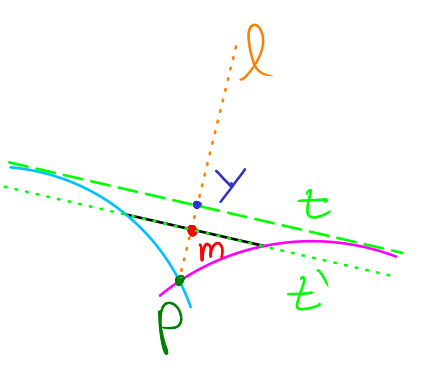
\includegraphics[width=0.4\textwidth]{8.png}
\end{figure}

The above algorithm determines an edge of the polygon $M$ given any starting position $x_0$ outside of $M$.
The next step is to discover the endpoints of a given edge.
We currently have four algorithms for determining an endpoint.
For the algorithms below, suppose that we have identified that an edge $e$ lies on the line $\ell$.
We will first find a point $x_0$ on $\ell$ that does not lie on $e$ by sampling points along $\ell$ with a given step size, until the oracle returns a value greater than zero.
Our goal is to find the endpoint $p$ of $e$ closest to $x_0$.

\textbf{Linear Search.}
Since $\F(x_0)>0$ we have a circle centered at $x_0$ that intersects the polytope $M$ at some point.
Note that this intersection point may not be on $e$, or even on an edge adjacent to $e$.
We will inductively construct a sequence of points converging to $p$.
Given a point $x_n$, we choose $x_{n+1}$ to be the intersection of the circle $S_n$ and $\ell$ closest to $M$ (as reported by the oracle).
Since each circle intersects $\ell$ exactly twice and we choose the point closest to $M$, the sequence approaches the endpoint $p$.

\begin{figure}[H]
	\centering
	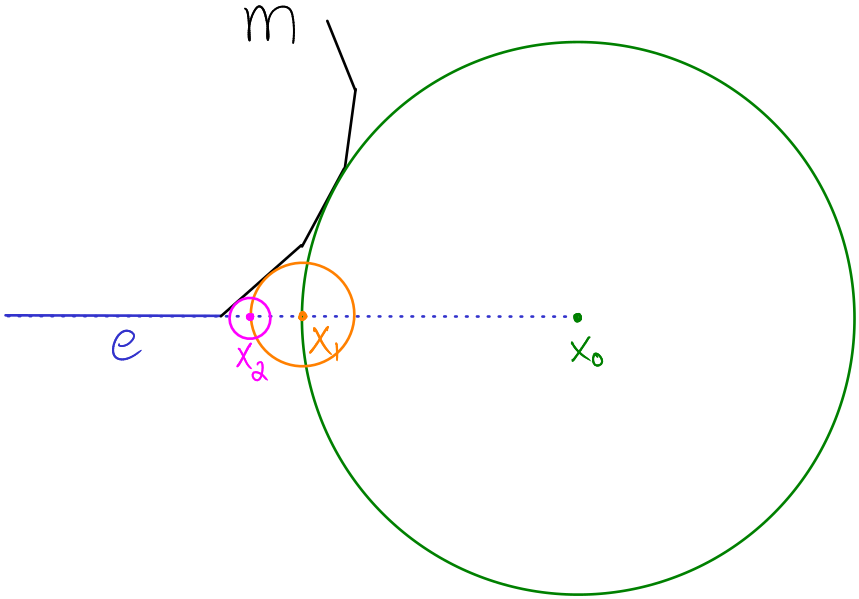
\includegraphics[width=0.6\textwidth]{binary.png}
\end{figure}

\textbf{Tangent Line I.}
Given $x_0$, we first choose the point $y_0$ to be the intersection of $S_{x_0}$ and $\ell$.
Let $t_{0}$ be any of the common tangent lines to both $S_{x_0}$ and $S_{y_0}$.
Since both $x_0$ and $y_0$ lie on $\ell$, the tangent $t_{0}$ intersects $\ell$ at a point $x_1$ closer to $M$ than $x_0$ and $y_0$.
We continue inductively to create a sequence converging to $p$.

Note that if the two points $x_n$ and $y_n$ used to generate the tangent $t_n$ lie in the domain of a common edge, then $t_n$ contains that edge.
In particular, if this edge is adjacent to $e$ then the next point in the sequence $x_{n+1}$ is exactly equal to $p$.

\begin{figure}[H]
	\centering
	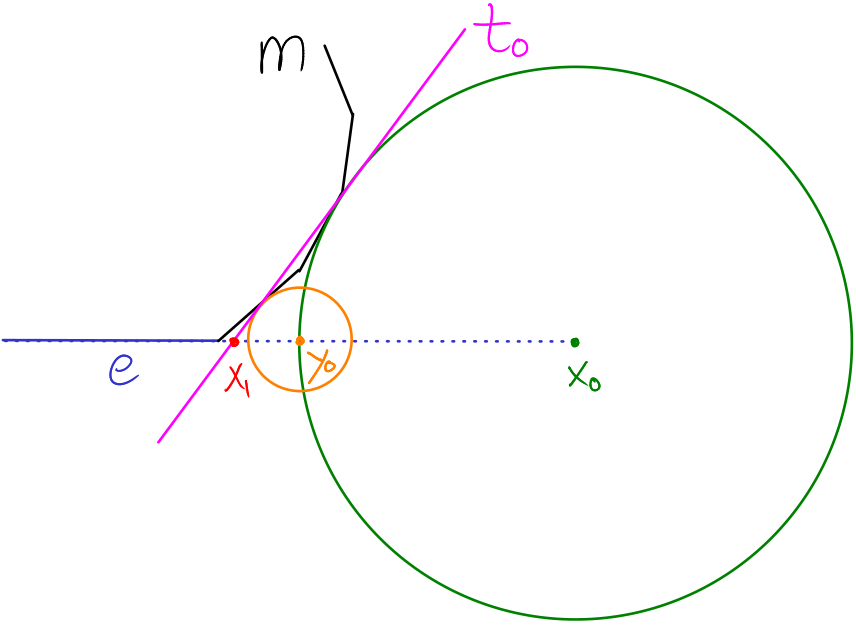
\includegraphics[width=0.6\textwidth]{tangent.png}
\end{figure}

\textbf{Tangent Line II.}
We employ the same technique as in the previous algorithm, but instead of choosing $y_n$ to be the intersection of $\ell$ and $S_{x_n}$, we use the point $x_0-\epsilon$ that is a distance of $\epsilon$ closer to $M$ than $x_n$.
The tangent line $t_n$ is constructed in the same fashion, as is the next point $x_{n+1}$ in the sequence.

\begin{figure}[H]
	\centering
	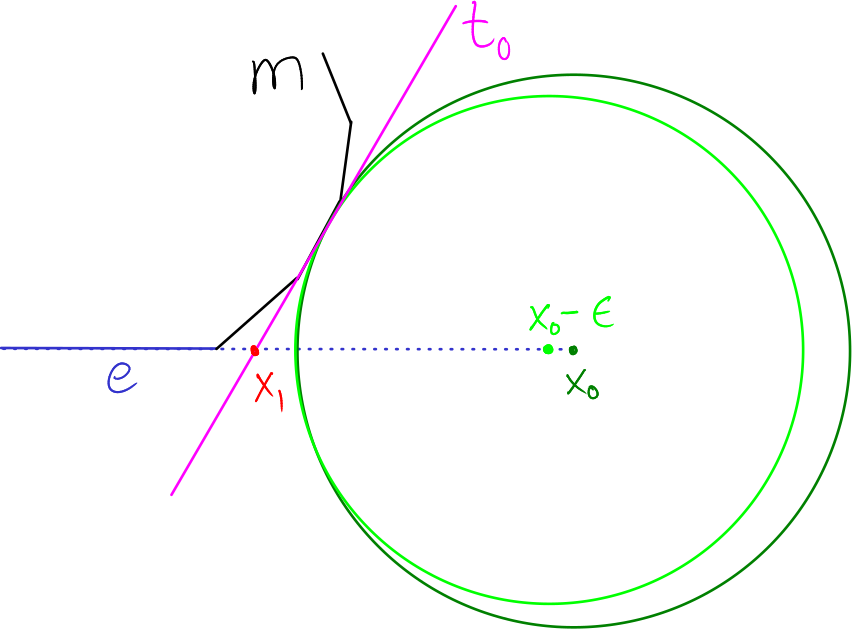
\includegraphics[width=0.6\textwidth]{inf_tangent.png}
\end{figure}

\textbf{Point Domain.}
Suppose the point $p$ is attached to the edges $e$ and $e'$.
The domain of $p$ is an open cone bounded by rays orthogonal to $e$ and $e'$ emanating from $p$ facing away from $M$.
Say that these rays $L$ and $L'$, respectively.

Consider a ray parallel to $L$ that starts at $x_0$.
We wish to find a point on this ray that is in the domain of $p$.
Since $M$ does not have any degenerate edges, this ray and $L'$ must intersect at some point $q$.
Points below $q$ with respect to the ray must the lie in the open cone representing $\dom(p)$.

If we assume that $\epsilon$ is the smallest unit of distance for our algorithm, then $1/\epsilon$ is the largest unit of distance. 
For small enough $\epsilon$, we may assume that the point $x_0-\frac{1}{\epsilon}$ found a distance of $1/\epsilon$ away from $x_0$ in the direction of the ray $L$ emanating from $x_0$ lies in the domain of $p$.

Let $d=\F(x_0-\frac{1}{\epsilon})$.
Since $L$ is orthogonal to $\ell$ we may then solve for the distance $a$ from $x_0$ to $p$ to be 
\[a = \sqrt{d^2-\frac{1}{\epsilon^2}}.\]
The point $p$ is then the point that is a distance of $a$ away from $x_0$ closer to $M$, as measured along $\ell$.

Note that if $\epsilon$ is not small enough, then the point $x_0-\frac{1}{\epsilon}$ may not be in $\dom(p)$.
However, we can identify the error by checking whether $\F(x_0-a)=0$.
If not, then we can either choose a point along the ray further than $x_0-\frac{1}{\epsilon}$, or take $x_1=x_0-a$ and repeat the process from $x_1$.



\section{Identifying the Polygon}

Once an edge and a vertex is found, we may easily find identify all edges and vertices of the polygon.
Let $p$ be a vertex on an edge $e$ contained in the line $\ell$.
Let $p+\epsilon$ be the point on $\ell$ a distance of $\epsilon$ away from $p$ that has a positive distance from $M$.
Then the next edge $e'$ containing $p$ is determined by the line tangent to $S_{p+\epsilon}$ that contains $p$.


\newpage

\section{New Strategy: Normal Lines}

In this section we will explore a new strategy that is more robust in higher dimensions.
This new procedure is iterative, seeking to produce finer and finer approximations of the polytope at each stage.

We will first demonstrate the idea of the algorithm in the two-dimensional case.
Let $p\in\R^2$ be a point in the interior of $M$ and let $y\in\R^2$ be in the exterior of $M$.
That is, $\F(p)<0$ and $\F(y)>0$.
We may obtain a point $q\in\partial M$ by performing a search (using the oracle) along the line segment between $p$ and $y$.
For now, let us assume that $q$ lies on an edge $e$.

\begin{figure}[H]
	\centering
	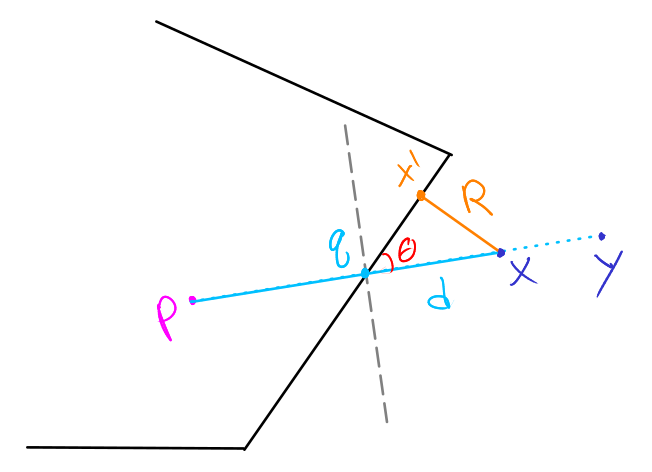
\includegraphics[width=0.6\textwidth]{2d.png}
\end{figure}

Now choose a point $x\in\R^2$ along the same line between $q$ and $y$ such that the distance between $q$ and $x$ is less than $\epsilon$.
We will then assume that $x$ being within $\epsilon$ of $q$ ensures that $x$ is in the domain of the edge that contains $q$.
Let $d$ be the distance between $q$ and $x$ and let $R=\F(x)$.
Suppose that the orthogonal projection of $x$ onto $e$ is the point $x'\in e$, so $R$ is the distance between $x$ and $x'$.

Since $x$ is in the domain of $e$, the points $q,x,x'$ determine a right triangle.
Let $\theta$ be the angle at $q$ with opposite side with length $R$ and with hypotenuse $d$.
We then have that $\theta=\cos^{-1}(R/d)$.
However, note that there are two possible unknown edge positions, corresponding to an angle of either $\theta$ or $\pi+\theta$.
The proper edge can be chosen by checking the oracle evaluation at a point on one of the possible edges;
consider a coordinate system with origin at $q$ and with one coordinate vector $e_1$ pointing from $q$ to $x$ and the other $e_2$ orthogonal to $e_1$.
Then the point
\[(\epsilon\cos\theta, \epsilon\sin\theta)\]
lies on one of the two possible edge configurations.

Now suppose that $q$ is a vertex of $M$.
We consider two cases: whether $x$ is in the domain of the vertex $q$ or in the domain of an edge $e'$.
Since $x$ is within $\epsilon$ of $q$, we will assume that $e'$ is an edge that contains $q$.
If $x\in\dom(e')$ then the algorithm proceeds as normal: since $e'$ contains $q$, we obtain a right triangle whose angle $\theta$ can be solved.
The resulting bounding line is the line that contains $e'$.
\begin{figure}[H]
	\centering
	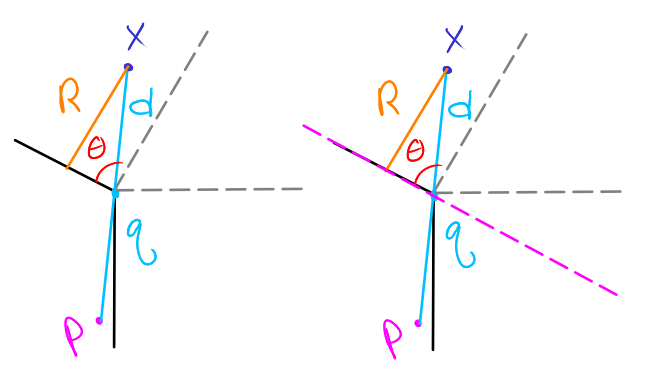
\includegraphics[width=0.6\textwidth]{vertex2.png}
\end{figure}
So assume that $x\in\dom(q)$, so $R=d$.
Since $M$ is convex, the interior angle at $q$ is less than $\pi$.
We may then take the line orthogonal to the line from $q$ to $x$ as our approximation of $M$. 
\begin{figure}[H]
	\centering
	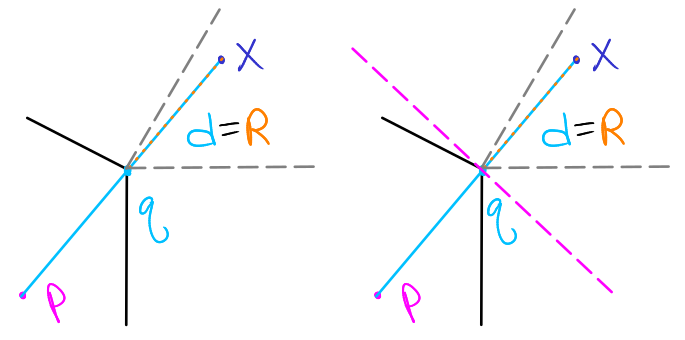
\includegraphics[width=0.6\textwidth]{vertex1.png}
\end{figure}

An iteration of the algorithm determines a bounding line $\ell$ for $M$.
By convexity, all of $M$ lies on one side of $\ell$.
Therefore, by running this algorithm over the four coordinate directions $\pm e_1,\pm e_2$, we obtain four bounding lines for $M$.
\begin{figure}[H]
	\centering
	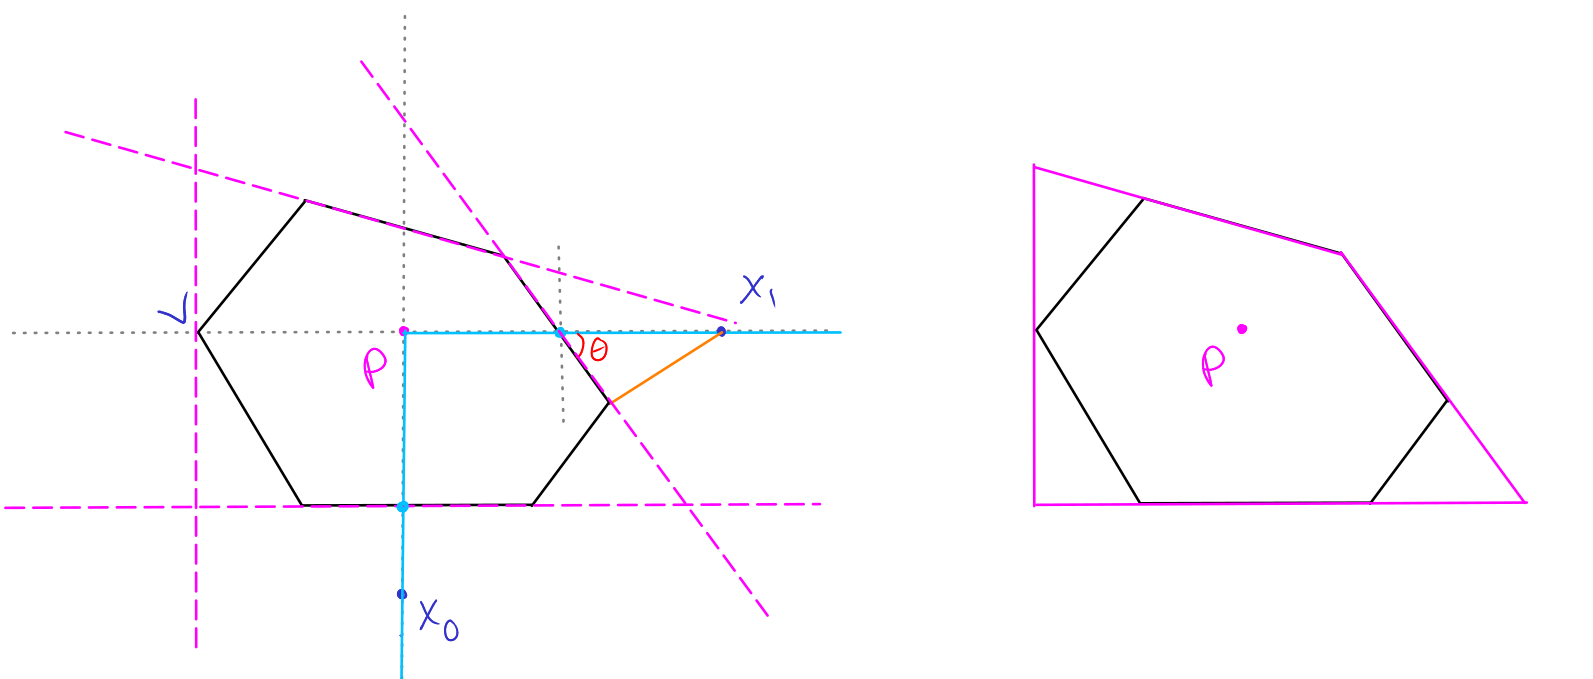
\includegraphics[width=0.6\textwidth]{complete.png}
\end{figure}

\textbf{Questions:}
\begin{itemize}
	\item Are the only problem points the vertices in the approximation?
		What about if all coordinate direction points were vertices?
	\item What happens in the case that the $\epsilon$ approximation fails?
		That is, when there are edges of length less than $\epsilon$ in each stage of the algorithm?
\end{itemize}

\subsection{Higher Dimensions}

The basic idea of the above algorithm generalizes to $n$ dimensions.
We may still choose points along each coordinate direction and search for points on the polytope.
We must find a more robust way of comparing distances with the oracle distance than using angles, as this does not generalize well to $\R^n$.

Let $M\subset\R^n$ be an $n$-dimensional convex polytope in $\R^n$.
Once again, let $p\in\R^n$ be a point in the interior of $M$ and $x\in\R^n$ be exterior to $M$.
Search for a point $q\in \partial M$ along the line segment containing $p$ and $x$.

Assume that $q$ lies in the interior of a (top-dimension) facet $F$ of $M$, and that all points within an $\epsilon$-ball of $x$ lie in the domain of $F$.
If $N=(N_1,\dots, N_n)$ is a normal vector to $F$ pointing to the exterior of $M$, then the distance from $x$ to $F$ is given by 
\[\F(x) = \frac{\ip{x-q,N}}{\abs{N}}=\bigip{x-q,\frac{N}{\abs{N}}}.\]
Note that our choice of $x$ on the exterior of $M$ ensures that this distance is positive.

Since all points in an $\epsilon$-neighborhood of $x$ lie within the domain of $F$, we can choose $n$ samples $\set{x_i}_{i=1}^n$ in this neighborhood whose distance to $F$ is given by 
\[\F(x_i) = \frac{\ip{x_i-q,N}}{\abs{N}}=\bigip{x_i-q,\frac{N}{\abs{N}}}.\]
We then have a linear system of $n$ equations in the $n$ unknown components of the unit normal vector $\frac{N}{\abs{N}}$ to the facet $F$.
Under the assumption that all points lie in the domain of $F$, the solution exists and is unique.
(A simple numerical experiment indicates that a solution for the \textit{unit} normal vector is readily found using samples chosen from a uniform distribution on an $\epsilon$-sphere surrounding $x$.
See \textit{experiment.py}.)

In the case that some of the samples $x_i$ are contained in the domains of different faces of $M$, the linear system will not have a unique solution.
Our original proposal to fix this issue is to simply choose the hyperplane containing $q$ that is orthogonal to the line from $p$ to $x$.
Unfortunately this technique does not always work, as shown by the figure below.
\begin{figure}[H]
	\centering
	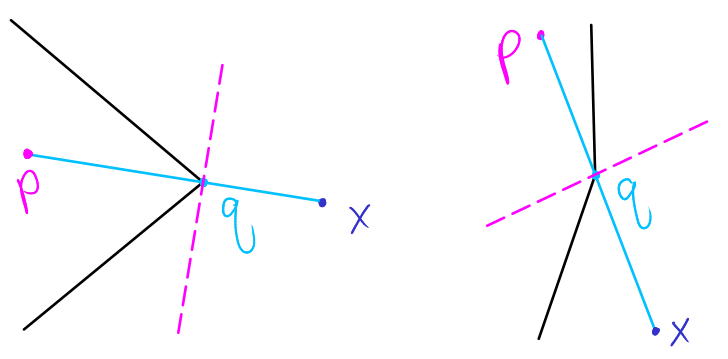
\includegraphics[width=0.6\textwidth]{vertex_issue.png}
	\caption{The dotted purple line is the chosen hyperplane at a vertex.
		Left: The orthogonal hyperplane is valid.
		Right: The orthogonal hyperplane is invalid.}
\end{figure}
We may solve this issue by changing the sampling strategy.
Rather than selecting random samples from an $\epsilon$-ball surrounding $x$, we pick samples along the line segment from $q$ to $x$ that are within $\epsilon$ of $q$.

Consider a ray $\ell$ emanating from a point $q$ of a face $F$ (of any dimension) of $M$.
There exists a neighborhood $U$ of $q$ on $\ell$ such that all points of $U$ are contained in the domain of the same face $F'$ of $M$.
The common face $F'$ is either equal to $F$ or is an adjacent face to $F$, as shown below.
\begin{figure}[H]
	\centering
	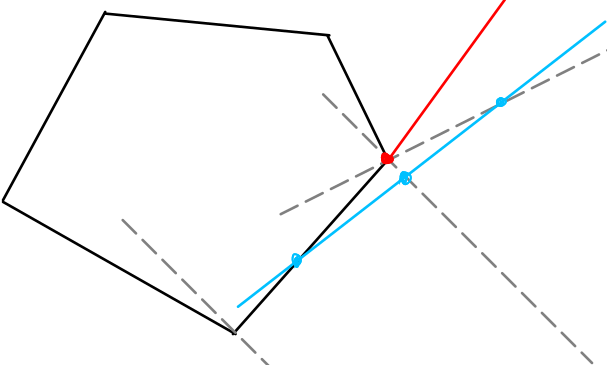
\includegraphics[width=0.6\textwidth]{ray_domain.png}
	\caption{Light blue: a ray that has a neighborhood contained in the original face domain.
	Red: a ray that has a neighborhood contained in an adjacent face domain.}
\end{figure}

We may use this fact to obtain a linear system of equations with a unique solution for any face $F$.
We still assume that we have a line segment from an interior point $p$ to an exterior point $x$, passing through a point $q\in\partial M$.
Let $U$ be the neighborhood of $q$ along the segment from $q$ to $x$ for which $U$ is in the domain of some face $F$ containing $q$.
Sample $n$ points $\set{x_i}_{i=1}^n$ in $U$, which all project to $F$ under the oracle.

Note that $F$ may not be a facet and so may not have a notion of normal vector, such as in the case of a vertex of a $2$-polytope.
However (needs proof for higher dimensions!) the distance function $\F$ of $U$ onto $F$ is equivalent to the orthogonal projection of $U$ onto some hyperplane containing $F$.
The unit normal of the hyperplane is directed into the domain of $F$ and so $M$ lies on the negative side of the hyperplane.
Therefore this hyperplane is a valid choice for generating a face of $Q_i$.
The figures below illustrate the choice of the hyperplane in $\R^2$.

\begin{figure}[H]
	\centering
	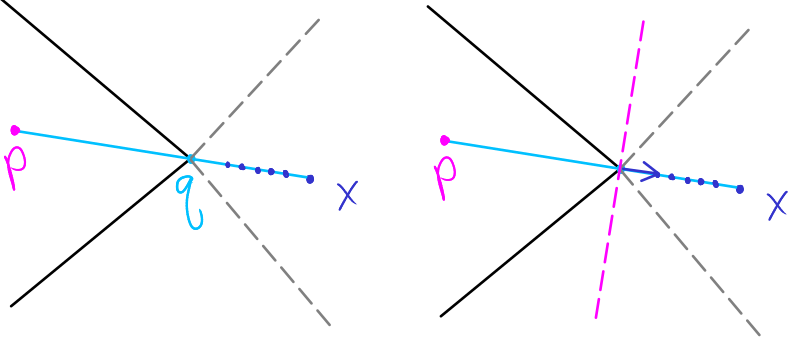
\includegraphics[width=0.6\textwidth]{vertex_fix.png}
	\caption{A common normal vector associated to a hyperplane containing a vertex.}
\end{figure}
\begin{figure}[H]
	\centering
	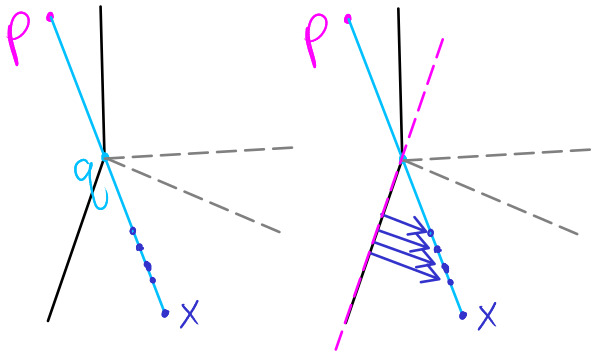
\includegraphics[width=0.6\textwidth]{facet_fix.png}
	\caption{A common normal vector associated to a hyperplane containing a hyperplane: results are consistent with the original algorithm for a facet.}
\end{figure}

The weakness of this strategy is the unknown neighborhood $U$.
Even with the assumption that $\epsilon$ is the minimum tolerance, the size of $U$ depends on the positions of $p$ and $x$.
In the figure below, the neighborhood $U$ may be very small in relation to the size of a face.
\begin{figure}[H]
	\centering
	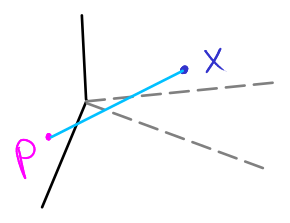
\includegraphics[width=0.3\textwidth]{epsilon_weakness.png}
\end{figure}
It is possible that this issue arises when $p$ is ``too close'' to a face.
One solution might be to more intelligently choose $p$ to be further in the interior of $M$, but it is unclear how this can be done.
Alternatively, we can reselect the point $x$ in some fashion.
However, this method fails in further iterations of the algorithm, when $x$ is a vertex of $Q_i$ and so cannot be reselected.










































\end{flushleft}
\end{document}
